%Modelo desenvolvido pelo discente Bruno Sávio Fichos do curso de Engenharia Mecânica do CEFET-MG
%Versao 2021.1

\documentclass[12pt,oneside, bibliography=totoc]{report}
\usepackage{definitions}
\usepackage{listings}
\pagestyle{plain}

\usepackage[
backend=biber,
style=alphabetic,
sorting=ynt
]{biblatex}
\addbibresource{refs.bib}


\lstset{ 
  language=Octave,                % the language of the code
  basicstyle=\footnotesize,       % the size of the fonts that are used for the code
  numbers=left,                   % where to put the line-numbers
  numberstyle=\tiny\color{gray},  % the style that is used for the line-numbers
  stepnumber=1,                   % the step between two line-numbers. If it's 1, each line 
                                  % will be numbered
  numbersep=5pt,                  % how far the line-numbers are from the code
  %backgroundcolor=\color{bg},    % choose the background color. You must add \usepackage{color}
  showspaces=false,               % show spaces adding particular underscores
  showstringspaces=false,         % underline spaces within strings
  showtabs=false,                 % show tabs within strings adding particular underscores
  frame=single,                   % adds a frame around the code
  rulecolor=\color{black},        % if not set, the frame-color may be changed on line-breaks within not-black text (e.g. commens (green here))
  tabsize=4,                      % sets default tabsize to 2 spaces
  captionpos=b,                   % sets the caption-position to bottom
  breaklines=true,                % sets automatic line breaking
  breakatwhitespace=false,        % sets if automatic breaks should only happen at whitespace
  title=\lstname,                 % show the filename of files included with \lstinputlisting;
                                  % also try caption instead of title
  keywordstyle=\color{blue}, %blue     % keyword style
  commentstyle=\color{dkgreen}, %dkgreen   % comment style
  stringstyle=\color{mauve}, %mauve      % string literal style
  escapeinside={\%*}{*)},         % if you want to add a comment within your code
  morekeywords={*,...}            % if you want to add more keywords to the set
    backgroundcolor=\color{backcolour},   
    commentstyle=\color{codegreen},
    numberstyle=\tiny\color{codegray},
    stringstyle=\color{codepurple},
    basicstyle=\ttfamily\footnotesize,
    breakatwhitespace=false,         
    breaklines=true,                 
    captionpos=b,                    
    keepspaces=true,                 
    numbers=left,                    
    numbersep=5pt,                  
    showspaces=false,                
    showstringspaces=false,
    showtabs=false,                  
    tabsize=2
}
\makeglossaries
\pagenumbering{gobble}
%%%%%%%%%%%%%%%%%%%%%%%%%%%%%%%%%%%%%%%%%%%%%%%%%%%%%%%%%%%%%
\usepackage{multicol}
\setlength{\columnsep}{1cm}
\definecolor{cefetblue}{RGB}{2, 65, 112}
\PassOptionsToPackage{pdftex}{graphicx}
\usepackage{graphicx}   
    
\usepackage[T1]{fontenc}
\usepackage[utf8]{inputenc} 
\usepackage[brazil]{babel}
\usepackage{epstopdf}
\usepackage{soul}
\usepackage{array}
\usepackage[table]{xcolor}  % 'table' option loads »colortbl«
\usepackage{lipsum}
\usepackage{subfig}
\RequirePackage[numbers]{natbib}
\usepackage{microtype} %melhor divisao de espaco entre letras/palavras
% aumentando as margens originais do documento
%\addtolength{\hoffset}{-1.5cm}
\usepackage{biblatex}

\usepackage{listings}
\usepackage{color}
\makeglossaries
%\newglossaryentry{latex}{   
%    name=latex,
%    description={Is a mark up language specially suited for scientific documents}
%}
 
\newglossaryentry{input}{   
    name=input,
    description={Informação ou dado que é utilizado como dado de entrada para um problema}
}

\newglossaryentry{output}{   
    name=output,
    description={Informação ou dado que é utilizado como dado de saída para um problema}
}



\newglossaryentry{overfitting, overfit, overfitted}{   
    name=overfitting,
    description={Superdimensionamento}
}


\newglossaryentry{underfitting, underfit, underfitted}{   
    name=overfitting,
    description={Subdimensionamento}
}










%%%%%%%%%%%%%%%%%%%%%%%%%%%%%%%%%%%%%%%%%%%%%%%%%%%%%%%%%%%%%%%%%%%

\newacronym{nvh}{NVH}{Noise, Vibration and Harshness}
\newacronym{frf}{FRF}{Função de Resposta em Frequência}
\newacronym{svd}{SVD}{Singular Value Decomposition}
\newacronym{si}{SI}{Sistema Internacional de Unidades}
\newacronym{ame}{AME}{Análise modal experimental}
\newacronym{am}{AM}{aprendizado de máquina}


%\acrlong{ }  \acrlong{gcd} prints Greatest Common Divisor.
%\acrshort{ } \acrshort{gcd} renders as GCD.
%\acrfull{ }  \acrfull{lcm} is Least Common Multiple (LCM).

%\Gls{latex} typesetting markup language is specially suitable for documents that include \gls{maths}. %\Glspl{formula} are rendered properly an easily once one gets used to the commands.
\makenomenclature
\usepackage{listings}
\usepackage{color}
\definecolor{codegreen}{rgb}{0,0.6,0}
\definecolor{codegray}{rgb}{0.5,0.5,0.5}
\definecolor{codepurple}{rgb}{0.58,0,0.82}
\definecolor{backcolour}{rgb}{0.95,0.95,0.92}
\addbibresource{refs.bib}
\definecolor{gray}{rgb}{0.5,0.5,0.5}
\definecolor{mauve}{rgb}{0.58,0,0.82}
\definecolor{bg}{rgb}{0.95,0.95,0.95}
\begin{document}
    
    \thispagestyle{empty}
\begin{center}

\begin{figure}
    \centering
    \hspace{-2.5cm}\begin{minipage}{.1\textwidth}
        
\includegraphics[width=2cm]{img/cefet.jpg}
        \end{minipage}\
    \hspace{0.75cm}
	\begin{minipage}{.8\textwidth}
	    \centering \large \textbf{\footnotesize{CENTRO FEDERAL DE EDUCAÇÃO TECNOLÓGICA DE MINAS GERAIS}}\\ \large{DEPARTAMENTO DE COMPUTAÇÃO}
        \end{minipage}\
    \hspace{0.45cm}
    \begin{minipage}{0.1\textwidth}
        
\includegraphics[width=3cm]{img/decom.png}
        \end{minipage}
\end{figure}


    \vspace{15mm}
    
    \begin{Large}
        \uppercase{\textbf{Implementação Compilador}}    
    \end{Large}
    \vspace{4cm}
    
    
    \uppercase{\textbf{\Large Analisador Sintático}

\end{center}

\vspace{6cm}

\begin{large}
        \flushleft{
            \textbf{Autor:} Alan Ferreira Leite Santos \\ Marcos Junio da Silva Xavier \\ Samuel Filipe dos Santos \\
            \textbf{Orientador:} Kecia Aline Marques Ferreira
 \\
        }
\end{large}

\vfill
\begin{center}
    \textbf{\large \monthyeardate\today, Belo Horizonte}
\end{center}
\clearpage

    \thispagestyle{empty}
\begin{center}


\begin{figure}
    \centering
    \hspace{-2.5cm}\begin{minipage}{.1\textwidth}
        
\includegraphics[width=2cm]{img/cefet.jpg}
        \end{minipage}\
    \hspace{0.75cm}
	\begin{minipage}{.8\textwidth}
	    \centering \large \textbf{\footnotesize{CENTRO FEDERAL DE EDUCAÇÃO TECNOLÓGICA DE MINAS GERAIS}}\\ \large{DEPARTAMENTO DE COMPUTAÇÃO}
        \end{minipage}\
    \hspace{0.45cm}
    \begin{minipage}{0.1\textwidth}
        
\includegraphics[width=3cm]{img/decom.png}
        \end{minipage}
\end{figure}


    \vspace{15mm}
    
    \begin{Large}
        \textbf{ Alan Ferreira Leite Santos \\ Marcos Junio da Silva Xavier \\ Samuel Filipe dos Santos }    
    \end{Large}
    \vspace{4cm}
    
    
    \uppercase{\textbf{\Large Implementação Compilador \\Parte I-   Analisador Léxico}}
\end{center}

\vspace{6cm}

\begin{flushright}
    \begin{minipage}{20em}%
        %\justify%
        Trabalho realizado em consonância com os princípios teóricos aprendidos durante o semestre a fim de criar, por etapas, um compilador para uma determinada linguagem proposta pela  orientadora.\\
        Orientador: Kecia Aline Marques Ferreira

    \end{minipage}

\end{flushright}


\vfill
\begin{center}
    \textbf{\large \monthyeardate\today, Belo Horizonte}
\end{center}
\clearpage

    %\thispagestyle{empty}
\begin{figure}
    \centering
    \hspace{-2.5cm}\begin{minipage}{.1\textwidth}
        
\includegraphics[width=2cm]{img/cefet.jpg}
        \end{minipage}\
    \hspace{0.75cm}
	\begin{minipage}{.8\textwidth}
	    \centering \large \textbf{\footnotesize{CENTRO FEDERAL DE EDUCAÇÃO TECNOLÓGICA DE MINAS GERAIS}}\\ \large{DEPARTAMENTO DE ENGENHARIA MECÂNICA}
        \end{minipage}\
    \hspace{0.45cm}
    \begin{minipage}{0.1\textwidth}
        
\includegraphics[width=3cm]{img/dem.png}
        \end{minipage}
\end{figure}

\vspace{2em}


\begin{justify}
Este Trabalho de Conclusão de Curso foi apresentado em XX de XXXXXX de 202X como requisito parcial para a obtenção do título de Bacharel em Engenharia Mecânica. O candidato foi arguido pela Banca Examinadora composta pelos profissionais abaixo assinados. Após deliberação, a Banca Examinadora considerou o trabalho aprovado.
\end{justify}
\begin{center}
    \vspace{3em}
    
    \begin{tabular}{@{}p{80mm}@{}}
        \hrulefill \\
        \centering Assinatura do Orientador \\
        \centering Nome do Orientador \\
        \vspace{2em}
        
        \hrulefill \\
        \centering Assinatura do Membro Titular da Banca \\
        \centering Nome do membro titular da banca \\
        \vspace{2em}
        
        \hrulefill \\
        \centering Assinatura do Membro Titular da Banca\\
        \centering Nome do membro titular da banca
    \end{tabular}

    \vfill
    \textbf{\large \the\year{} Belo Horizonte}
\end{center}
\clearpage

    %\include{tcc1/parte1}
    %\include{tcc1/parte2}
    %\include{tcc1/parte3}
    %\thispagestyle{empty}

\vspace*{\fill}

\begin{flushright}
    \begin{minipage}{20em}%
        %\justify%
    A todos que ajudam o CEFET-MG se tornar melhor a cada dia.
    \end{minipage}

\end{flushright}


\clearpage

    %\thispagestyle{empty}

\begin{center}
\uppercase{\textbf{\large{Agradecimentos}}}
\end{center}

agradecimentos, ....


\clearpage

    
  \clearpage
    \begin{center}
\uppercase{\textbf{\large{Resumo}}}
\end{center}
Na disciplina de Compiladores, ofertada pelo CEFET-MG, iremos construir um compilador ao longo do semestre, este, dividido em etapas. Na primeira etapa, entregamos a implementação do analisador léxico e a Tabela de Símbolos em Java. Nesta segunda etapa, estamos entregando a analise do programa levando em consideração a derivação da linguagem.Tais conhecimentos obtidos com a disciplina orientados pela Dr Kecia Ferreira, para que seja possível, utilizamos como base os conceitos abordados pelo Aho, em seu livro : "Compiladores Princípios ,Técnicas e Ferramentas"
\vspace{2cm}

\textbf{Palavras Chaves:} java,compilador

\vfill
\clearpage
    \begin{center}
\uppercase{\textbf{\large{Abstract}}}
\end{center}

In the course of Compilers, offered by CEFET-MG, we will build a compiler throughout the semester, this one, divided into stages. In this first stage, we are delivering the Java implementation of the lexical analyzer and the Symbol Table, knowledge obtained with the discipline guided by Dr Kecia Ferreira, to make it possible, we use as a basis the concepts covered by Aho, in his book: "Compilers Principles, Techniques and Tools"
\vspace{5cm}

\textbf{Key-words:} java,compiler

\clearpage
        \listoffigures
    \pagebreak
    \listoftables
    \printglossary[type=\acronymtype]
    \printglossary
    \printnomenclature
    \clearpage
    
    \tableofcontents{}
    \clearpage
    \setcounter{page}{1}
    \pagenumbering{arabic}
 
    \chapter{Introdução}

Um compilador é um programa de computador (ou um grupo de programas) que, a partir de um código fonte escrito em uma linguagem compilada, cria um programa semanticamente equivalente, porém escrito em outra linguagem, código objeto. Classicamente, um compilador traduz um programa de uma linguagem textual facilmente entendida por um ser humano para uma linguagem de máquina , específica para um processador e sistema operacional. Atualmente, porém, são comuns compiladores que geram código para uma máquina virtual que é, depois, interpretada por um interpretador. Ele é chamado compilador por razões históricas; nos primeiros anos da programação automática, existiam programas que percorriam bibliotecas de sub-rotinas e as reunia, ou compilava, as sub-rotinas necessárias para executar uma determinada tarefa.

O nome "compilador" é usado principalmente para os programas que traduzem o código fonte de uma linguagem de programação de alto nível para uma linguagem de programação de baixo nível (por exemplo, Assembly ou código de máquina). Contudo alguns autores citam exemplos de compiladores que traduzem para linguagens de alto nível como C. Para alguns autores um programa que faz uma tradução entre linguagens de alto nível é normalmente chamado um tradutor, filtro ou conversor de linguagem. Um programa que traduz uma linguagem de programação de baixo nível para uma linguagem de programação de alto nível é um descompilador. Um programa que faz uma tradução entre uma linguagem de montagem e o código de máquina é denominado montador (assembler). Um programa que faz uma tradução entre o código de máquina e uma linguagem de montagem é denominado desmontador (disassembler). Se o programa compilado pode ser executado em um computador cuja CPU ou sistema operacional é diferente daquele em que o compilador é executado, o compilador é conhecido como um compilador cruzado.
    
\chapter{Palavras Reservadas}
Para que o compilador seja executado de forma correta, existem algumas regrinhas a serem seguidas, uma delas é a definição de palavras reservadas, essas, são palavras que não devem ser utilizadas em nenhum outro momento a não ser o que foi pre-determinado pelos programadores da linguagem.
Como por exemplo: No caso deste compilador, existe a palavra stop, a qual significa que quando o compilador ler esse token, significa que o programa chegou ao final, logo, em nenhum outro local esse token deve ter outro significado a não ser o significado que já foi determinado. Não se pode atribuir uma outra função a uma palavra reservada.
 \begin{table}[H]
        \vspace{1.0em}
        \centering%
        \caption{Relação das Palavras Reservadas da Linguagem}%
        \begin{tabular} {p{5cm}p{11cm}}% Aqui é possível definir o tamanho de cada coluna. 
            \hline
            \textbf{Palavra Reservada}  & \textbf{Significado}\\
            \hline
            {init}             &   {Inicio do Programa}   \\
            \hline
            {stop}&{Indica a finalização do programa }\\
            \hline
            {is} & {Usado para determinador o tipo de uma variável} \\
            \hline
            

{integer}&{Tipo Inteiro para variável} \\
              \hline
{string}&{Determina a variável como tipo string}\\
  \hline
{real} & {Determina a variável como tipo Real} \\
\hline


{if}&{Determina o inicio de um bloco de código sob uma condicional}\\
\hline

{begin}&{Deternia o inicio de uma condição do if}\\
\hline
{end}&{Determina o fim da condição do if}\\
\hline
{else}&{Determina a contraposição da condição do if}\\
\hline
{end else}&{Indica o Fim da condição do Else if}\\
\hline
{do}&{Determina a entrada de um laço }\\
\hline
{while}&{determina a condição para o laço Do}\\
\hline
{read}&{Prepara para ler e reservar a próxima variável a ser lida}\\
\hline
{write}&{Determina que ira imprimir na tela a literal que virá a seguir}\\
\hline
{not}&{Determina a negação do valor booleano de uma expressão}\\
\hline
{or}&{Determina a soma binaria entre dois valores }\\
\hline
{and}&{Determina a multiplicação binaria entre dois valores}\\

            \hline
        \end{tabular}
        \\\hspace{\linewidth}%
        \textbf{Fonte:} Documentação Fornecida pela Orientadora o qual pode ser consultado no diretório do projeto%
        \label{table:cronograma}
        \vspace{1.0em}
    \end{table}

\begin{center} \printglossaries
\end{center}
    \chapter{Melhorias Gradativas}
Para iniciar o desenvolvimento dessa segunda parte do trabalho que faz parte do desenvolvimento do compilador, tivemos que consertar erros que foram relatados na parte anterior (Analisador Léxico) pela nossa orientadora Kecia.
Foram pontuados os seguintes erros:

\begin{itemize}
    \item 
       O resultado do Teste 1 mostrado não corresponde a ele. -0,25.
    \item
        Teste 4: não reconheceu o erro de comentário não fechado. -0,25
    \item
        Teste 2: "{\_}valor" tem que ser reportado como erro. -0,25
    \item
    Faltou o Teste 5. -0,25
   \end{itemize}
Esses erros passaram desapercebidos e foram corrigidos para essa entrega do trabalho.
    \chapter{Forma de Utilização}
\usepackage{}
Para que seja possível a utilização deste programa, basta entrar no terminal e navegar até o diretório: "TP{\_}Compilador/src/", e então, digitar o seguinte comando :
\begin{lstlisting}[language=Java, caption={Entrada terminal},label={Terminal para inicio do Programa}]
    javac Main.java
    java Main
\end{lstlisting}
Acima podemos ver duas linhas de comando, a primeira serve para que possa compilar a classe Main.java e então, é criado o executável e assim, podemos acessar a classe a partir da linha seguinte, java Main .
\newline
Definimos qual arquivo de teste que o programa deve compilar dentro da classe Main, no seguinte trecho de código:
\begin{lstlisting}[language=Java, caption={Indicando arquivo para teste},label={Terminal para inicio do Programa}]
public class Main {
	public static void main(String[] args) {
		ArrayList<Token> tokens = new ArrayList<Token> ();
		Lexer L = null;
		int line = -5;
		try {
			L = new Lexer("codigos_teste/corretos/Teste1.txt");
			L.adicionapalavras();//Inicia adicionando palavras reservadas
			System.out.println("**** Tokens lidos ****");
			// Apenas para entrar no laço
			Token T = new Token(0, line);
			while (T.tag != Tag.EOF) {
				try {
					T = L.scan();
					if(T.tag == Tag.EOF)
						break;
					T.imprimeToken(T);
					tokens.add(T);
					line = T.line;
				} catch (InvalidTokenException | IOException e) {
					System.out.println(e.getMessage());
					try {
						L.readch();
					} catch (IOException e1) {
						e1.printStackTrace();
					}
				}
			}
			line++;
			tokens.add(new Token(Tag.EOF, line));
			//L.imprimirTabela();
			Parser P = new Parser(tokens);
			System.out.println("\n\n\n**** Inicio Parser ****");
			P.init();
		} catch (FileNotFoundException e) {
			e.printStackTrace();
		}
	}
}
			
\end{lstlisting}
\newline 
Na linha 7 (sete) do trecho do código destacado acima, mostra como determinamos qual programa nosso compilador irá testar.
Veja que criamos uma pasta chamada testes para que seja incluídos somente os arquivos de teste do programa. Foram criados 10 arquivos de teste.





    \chapter{Documentação}
O Analisador Sintático tem a função de solicitar ao Analisador léxico o próximo Tokens desde o inicio do programa ate o final, e apos a cada solicitação, verificar se o Token lido esta em consonância com o que foi determinado pela gramatica do programa.
\newline
O Projeto foi desenvolvido em conjunto com as plataformas Visual Studio Code e Apache Netbeans, a principio todo o código seria criado somente "a mão" criando as pastas e arquivos manualmente, porém, devido a algumas facilidades que o Netbeans  oferece, o projeto foi alterado em alguns parâmetros para que seja possível abrir no Netbeans.
Uma dessas facilidades é a opção de geração da Documentação do projeto, assim o fizemos e esta documentação gerada automaticamente pelo Netbeans se encontra no diretório: " /TP{\_}Compilador/Projeto/dist/javadoc/" . Para esta implementação foi acatado o modelo abordado pelo autor do livro base da disciplina: Aho .
\section{Tabela Frist-Follow e LL(1)}

Para evitar o retrocesso métodos baseados em 
tabela são utilizados. Para auxiliar na construção 
das tabelas sintáticas deve serutilizado as funções first(α)
e follow(A)
\subsection{Frist}

Defina First(α), onde α é qualquer cadeia de 
símbolos da gramática, como sendo o conjunto 
de símbolos terminais que iniciam as cadeias 
derivadas de α. Se α → * ε, então ε está no 
First(α)
\subsection{Calculando Frist(X)}

Para calcular o First(X) para todo símbolo X da 
gramática, aplique as seguintes regras até que não haja 
mais terminais ou e que possam ser acrescentados a 
algum dos conjuntos First.


\begin{itemize}
    \item 
       Se X é um símbolo terminal, então First(X)= {X}
    \item
        Se X é um símbolo não-terminal e X → Y
1
Y
2
..Y
k
 é 
uma produção para k ≥ 1, então acrescente a ao 
First(X) se, para algum i, a  estiver em First( Y\i ), e ε
estiver em todos os First(Y\1),...,First(Y\i-1); ou seja,Y\1
...Y\i-1 → ε. Se ε está em First(Y\ j ) para todo j=1, 2, …, k então ε está em First(X).

    \item
       Se X → e é uma produção de X então ε está em  First(X).
    
   \end{itemize}
\section{Follow(A)}

Defina Follow(A), para o não-termianl A, como 
sendo o conjunto de terminais a que podem 
aparecer imediatamente à direita de A em uma 
forma sentencial; ou seja, o conjunto de terminais 
a tais que exista uma derivação na forma S → 
αAaβ, para algum α, β.
\subsection{Calculando Follow(A)}

Para calcular o Follow(A) para todos os nãoterminais da gramática aplique as seguintes 
regras até que nada mais possa ser 
acresncentado a nenhum dos conjuntos Follow

   
\begin{itemize}
    
       \item  Coloque {\$} (símbolo de final de cadeia) em 
Follow(S), onde S é o símbolo inicial da 
gramática.
\item
 Se houver uma produção A → αBβ, então tudo 
no First(β) exceto ε está em Follow(B).
\item
Se houver uma produção A → αB, ou uma 
produção A → αBβ onde Firts(β) contém ε , 
então inclua Follow(A) ao Follow(B).
   \end{itemize}
   
   
\section{LL(1)}

Análise LL(1)
   
\begin{itemize}
\item Conceitualmente, o analisador LL(1) constrói uma derivação mais à esquerda
para o programa, partindo do símbolo inicial
\item A cada passo da derivação, o prefixo de terminais da forma sentencial tem 
que casar com um prefixo da entrada
\item Caso exista mais de uma regra para o não-terminal que vai gerar o próximo 
passo da derivação, o analisador usa o primeiro token após esse prefixo para 
escolher qual regra usar

\item Esse processo continua até todo o programa ser derivado ou acontecer um 
erro (o prefixo de terminais da forma sentencial não casa com um prefixo do 
programa)

   \end{itemize}
   Assim, foi criado as tabelas de Frist e Follow da Gramatica e estao dispostas no arquivo Criado pelo Programa Microsoft Excel.
   O Arquivo encontra-se na pasta raiz deste trabalho,pode ser encontrado pelo nome : "AnaliseSintatica\_FristFollow\_LL1"
   
   
    \chapter{Planejamento}
Para que todo projeto possa ser bem sucedido, devem se analisar, projetar e estudar minuciosamente e fazer o levantamento de todo os requisitos necessários para o projeto.
Apartir das matérias de Modelagem e Desenvolvimento de Sistenas e Engenharia de Software, foi possível adquirir conhecimentos para um bom planejamento do trabalho.
Como esse trabalho demonstrou ser extenso e complexo, decidimos por nos planejarmos a fim de evitar que possíveis erros de implementação fosse acarretado durante a fase de Desenvolvimento.
Assim, fizemos uma reunião inicial para decidir os pontos importantes e decidir pontos sobre implementação do código.
Utilizamos um organizador de tarefas no Excel para acompanhar as tarefas.Tal diagrama sera utilizado para as próximas etapas também.
Veja abaixo, como ficou a organização do planejamento deste trabalho na figura abaixo.

\begin{figure}[H]
    \vspace{1.0em}
    \centering
    \caption{Planejamento Analise TP Compiladores}
    \subfloat[Diagrama Planejamento]{ % titulo da subimagem
        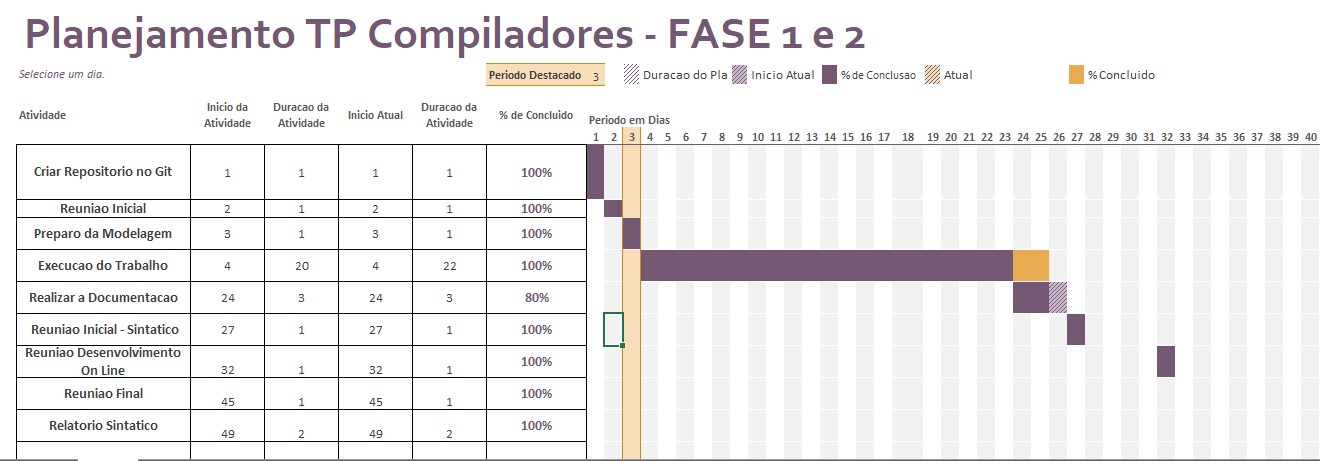
\includegraphics[width=1.0\textwidth]{img/Planejamento.jpg}%
        \label{fig:pendulo_movimento}
    }
 
    \hspace{\linewidth}%
    \textbf{Fonte:} Desenvolvedores do Código
    \label{fig:cefets}
    \vspace{1.0em}
\end{figure}
Tal arquivo se encontra dentro do diretório deste projeto criado pelo Programa Microsoft Excel, podendo ser acesso pelo caminho: "TP{\_}Compilador/Planejamento/"
    \chapter{Testes realizados}
Para testar todo o compilador construído, foram propostos sete exemplos de teste, abordando algumas possibilidade de programas a serem compilados.
Apartir desses arquivos podemos visualizar os seguintes retorno do compilador :
\newline



\begin{lstlisting}[caption={Teste1.txt},label={lst:label},language=Comsol]

init
a, b, $c, is integer;
result is real;
write("Digite o valor de a:"
read (a);
write("Digite o valor de c:"
read (c);
b := 10
result := (a * c)/(b + 5 - 345);
write("O resultado e:");
write(result);
stop


\end{lstlisting}\newline
Para o codigo acima  o compilador obeteve a seguinte saida :

\begin{lstlisting}[caption={Saida para o Codigo de teste  : Teste1.txt},label={Entrada 1},language=Comsol]
**** Tokens lidos ****
< identifier, a >
< virgula >
< virgula >
< identifier, b_1 >
< virgula >
< identifier, b_2 >
< virgula >
< identifier, cc >
< virgula >
< num, 10 >
Error(1): Token ' ' inválido
Error(1): Token ':' inválido
< integer_type >
< ponto_virgula >
< init_program >
< write >
< abre_parent >
< literal, "Entre com o valor de a:" >
< fecha_parent >
< ponto_virgula >
< read >
< abre_parent >
< identifier, a >
< fecha_parent >
< ponto_virgula >
< identifier, b_1 >
< assign >
< identifier, a >
< mult_mulop >
< identifier, a >
< ponto_virgula >
< write >
< abre_parent >
< literal, "O valor de b1 e:" >
< fecha_parent >
< ponto_virgula >
< write >
< abre_parent >
< identifier, b_1 >
< fecha_parent >
< ponto_virgula >
< identifier, b_2 >
< equal_relop >
< identifier, b >
< soma_addop >
< identifier, a >
< div_mulop >
< num, 2 >
< mult_mulop >
< abre_parent >
< identifier, a >
< soma_addop >
< num, 5 >
< fecha_parent >
< ponto_virgula >
< write >
< abre_parent >
< literal, "O valor de b1 e:" >
< fecha_parent >
< ponto_virgula >
< identifier, Write >
< abre_parent >
< identifier, b1 >
< fecha_parent >
< ponto_virgula >
< stop_program >



**** Tabela de símbolos ****
Entrada         |               Mais info
string
Write
not
end
is
b1
or
b_2
b_1
real
if
cc
while
do
stop
read
init
else
integer
write
begin
b
a
and


\end{lstlisting}\newline


\begin{lstlisting}[caption={Teste2.txt},label={lst:label},language=Comsol]
a, _valor, b_1, b_2, cc, 10_a : integer;
init
write("Entre com o valor de a:");
read (a);
b_1 := a * a;
write("O valor de b1 e:");
write (b_1);
b_2 = b + a/2 * (a + 5);
write("O valor de b1 e:");
Write (b1);
stop


\end{lstlisting}\newline

Para o codigo acima o compilador obeteve a seguinte saida :

\begin{lstlisting}[caption={Saida para o Codigo de teste  : Teste1.txt},label={Entrada 1},language=Comsol]
-------Tokens Reconhecidos pelo Compilador-------
< identifier, a >
< virgula >
< virgula >
< identifier, b_1 >
< virgula >
< identifier, b_2 >
< virgula >
< identifier, cc >
< virgula >
< num, 10 >
Error(1): Token ' ' inválido
Error(1): Token ':' inválido
< integer_type >
< ponto_virgula >
< init_program >
< write >
< abre_parent >
< literal, "Entre com o valor de a:" >
< fecha_parent >
< ponto_virgula >
< read >
< abre_parent >
< identifier, a >
< fecha_parent >
< ponto_virgula >
< identifier, b_1 >
< assign >
< identifier, a >
< mult_mulop >
< identifier, a >
< ponto_virgula >
< write >
< abre_parent >
< literal, "O valor de b1 e:" >
< fecha_parent >
< ponto_virgula >
< write >
< abre_parent >
< identifier, b_1 >
< fecha_parent >
< ponto_virgula >
< identifier, b_2 >
< equal_relop >
< identifier, b >
< soma_addop >
< identifier, a >
< div_mulop >
< num, 2 >
< mult_mulop >
< abre_parent >
< identifier, a >
< soma_addop >
< num, 5 >
< fecha_parent >
< ponto_virgula >
< write >
< abre_parent >
< literal, "O valor de b1 e:" >
< fecha_parent >
< ponto_virgula >
< identifier, Write >
< abre_parent >
< identifier, b1 >
< fecha_parent >
< ponto_virgula >
< stop_program >



------------- Imprimindo a Tabela de símbolos-------------
                Entrada
string
Write
not
end
is
b1
or
b_2
b_1
real
if
cc
while
do
stop
read
init
else
integer
write
begin
b
a
and

\end{lstlisting}\newline

\begin{lstlisting}[caption={Teste3.txt},label={lst:label},language=Comsol]
% Programa de Teste
Calculo de idade%
INIT
cont is int;
media, idade, soma is integer;
begin
cont := 5;
soma := 0;
do
write("Altura:" );
read (altura);
soma := soma+altura;
cont := cont - 1;
while(cont > 0)
media := soma / qts
write("Media: ");
write (media);
STOP
\end{lstlisting}


Para o codigo acima o compilador obeteve a seguinte saida :

\begin{lstlisting}[caption={Saida para o Codigo de teste  : Teste3.txt},label={Entrada 1},language=Comsol]

-------Tokens Reconhecidos pelo Compilador-------
< identifier, INIT >
< identifier, cont >
< is_decl >
< identifier, int >
< ponto_virgula >
< identifier, media >
< virgula >
< identifier, idade >
< virgula >
< identifier, soma >
< is_decl >
< integer_type >
< ponto_virgula >
< begin >
< identifier, cont >
< assign >
< num, 5 >
< ponto_virgula >
< identifier, soma >
< assign >
< num, 0 >
< ponto_virgula >
< do >
< write >
< abre_parent >
< literal, "Altura:" >
< fecha_parent >
< ponto_virgula >
< read >
< abre_parent >
< identifier, altura >
< fecha_parent >
< ponto_virgula >
< identifier, soma >
< assign >
< identifier, soma >
< soma_addop >
< identifier, altura >
< ponto_virgula >
< identifier, cont >
< assign >
< identifier, cont >
< menos_addop >
< num, 1 >
< ponto_virgula >
< while >
< abre_parent >
< identifier, cont >
< greater_than_relop >
< num, 0 >
< fecha_parent >
< identifier, media >
< assign >
< identifier, soma >
< div_mulop >
< identifier, qts >
< write >
< abre_parent >
< literal, "Media: " >
< fecha_parent >
< ponto_virgula >
< write >
< abre_parent >
< identifier, media >
< fecha_parent >
< ponto_virgula >
< identifier, STOP >



------------- Imprimindo a Tabela de símbolos-------------
                Entrada
STOP
string
int
INIT
cont
not
end
altura
idade
media
is
or
qts
soma
real
if
while
do
stop
read
init
else
integer
write
begin
and
\end{lstlisting}


\begin{lstlisting}[caption={Teste4.txt},label={lst:label},language=Comsol]
init
% Outro programa de teste
i, j, k, @total is integer;
nome is string
write("Digite o seu nome: ");
read(nome);
write("Digite um valor inteiro: );
read (I);
k := i * (5-i * 50 / 10;
j := i * 10;
k := i* j / k;
k := 4 + a $;
write(nome);
write(", os números gerados sao: ");
write(i);
write(j);
write(k);

\end{lstlisting}

Para o codigo acima o compilador obeteve a seguinte saida :

\begin{lstlisting}[caption={Saida para o Codigo de teste  : Teste4.txt},label={Entrada 1},language=Comsol]
-------Tokens Reconhecidos pelo Compilador-------
< init_program >
< mult_mulop >
< abre_parent >
< num, 5 >
< menos_addop >
< identifier, i >
< mult_mulop >
< num, 50 >
< div_mulop >
< num, 10 >
< ponto_virgula >
< identifier, j >
< assign >
< identifier, i >
< mult_mulop >
< num, 10 >
< ponto_virgula >
< identifier, k >
< assign >
< identifier, i >
< mult_mulop >
< identifier, j >
< div_mulop >
< identifier, k >
< ponto_virgula >
< identifier, k >
< assign >
< num, 4 >
< soma_addop >
< identifier, a >
Error(12): Token '$' inválido
< ponto_virgula >
< write >
< abre_parent >
< identifier, nome >
< fecha_parent >
< ponto_virgula >
< write >
< abre_parent >
< literal, ", os números gerados sao: " >
< fecha_parent >
< ponto_virgula >
< write >
< abre_parent >
< identifier, i >
< fecha_parent >
< ponto_virgula >
< write >
< abre_parent >
< identifier, j >
< fecha_parent >
< ponto_virgula >
< write >
< abre_parent >
< identifier, k >
< fecha_parent >
< ponto_virgula >



------------- Imprimindo a Tabela de símbolos-------------
                Entrada
string
not
end
is
or
real
if
while
do
stop
k
nome
j
read
i
init
else
integer
write
begin
a
and

\end{lstlisting}

\begin{lstlisting}[caption={Teste6.txt},label={lst:label},language=Comsol]
init
a, b, c, maior is integer;
write("Digite uma idade: ");
read(a);
write("Digite outra idade: ");
read(b);
write("Digite mais uma idade: ");
read(c;
maior := 0;
if ( a>b and a>c )
maior := a;
else
if (b>c)
maior := b;
else
maior := c;
write("Maior idade: ");
write(maior);
end

\end{lstlisting}

Para o codigo acima o compilador obeteve a seguinte saida :

\begin{lstlisting}[caption={Saida para o Codigo de teste  : Teste6.txt},label={Entrada 1},language=Comsol]
-------Tokens Reconhecidos pelo Compilador-------
< init_program >
< identifier, a >
< virgula >
< identifier, b >
< virgula >
< identifier, c >
< virgula >
< identifier, maior >
< is_decl >
< integer_type >
< ponto_virgula >
< write >
< abre_parent >
< literal, "Digite uma idade: " >
< fecha_parent >
< ponto_virgula >
< read >
< abre_parent >
< identifier, a >
< fecha_parent >
< ponto_virgula >
< write >
< abre_parent >
< literal, "Digite outra idade: " >
< fecha_parent >
< ponto_virgula >
< read >
< abre_parent >
< identifier, b >
< fecha_parent >
< ponto_virgula >
< write >
< abre_parent >
< literal, "Digite mais uma idade: " >
< fecha_parent >
< ponto_virgula >
< read >
< abre_parent >
< identifier, c >
< ponto_virgula >
< identifier, maior >
< assign >
< num, 0 >
< ponto_virgula >
< if >
< abre_parent >
< identifier, a >
< greater_than_relop >
< identifier, b >
< and_mulop >
< identifier, a >
< greater_than_relop >
< identifier, c >
< fecha_parent >
< identifier, maior >
< assign >
< identifier, a >
< ponto_virgula >
< else >
< if >
< abre_parent >
< identifier, b >
< greater_than_relop >
< identifier, c >
< fecha_parent >
< identifier, maior >
< assign >
< identifier, b >
< ponto_virgula >
< else >
< identifier, maior >
< assign >
< identifier, c >
< ponto_virgula >
< write >
< abre_parent >
< literal, "Maior idade: " >
< fecha_parent >
< ponto_virgula >
< write >
< abre_parent >
< identifier, maior >
< fecha_parent >
< ponto_virgula >
< end >



------------- Imprimindo a Tabela de símbolos-------------
                Entrada
string
maior
not
end
is
or
real
if
while
do
stop
read
init
else
integer
write
c
begin
b
a
and

\end{lstlisting}
\begin{lstlisting}[caption={Teste7.txt},label={lst:label},language=Comsol]
% Programa de Teste%
Calculo de idade
init
	cont_ is int;
	media, idade, soma_ is integer;
begin
	cont_ = 5;
	soma = 0;

	do
		write(“Altura:” );
		read (altura);
		soma := soma altura;
		cont_ := cont_ - 1;
	while(cont_ > 0)

	write(“Media: ”);
	write (soma / qtd);

stop
\end{lstlisting}

Para o codigo acima o compilador obeteve a seguinte saida :

\begin{lstlisting}[caption={Saida para o Codigo de teste  : Teste7.txt},label={Entrada 1},language=Comsol]
-------Tokens Reconhecidos pelo Compilador-------
< identifier, Calculo >
< identifier, de >
< identifier, idade >
< init_program >
< identifier, cont_ >
< is_decl >
< identifier, int >
< ponto_virgula >
< identifier, media >
< virgula >
< identifier, idade >
< virgula >
< identifier, soma_ >
< is_decl >
< integer_type >
< ponto_virgula >
< begin >
< identifier, cont_ >
< equal_relop >
< num, 5 >
< ponto_virgula >
< identifier, soma >
< equal_relop >
< num, 0 >
< ponto_virgula >
< do >
< write >
< abre_parent >
Error(11): Token '“' inválido
< identifier, Altura >
Error(11): Token ':' inválido
< fecha_parent >
< ponto_virgula >
< read >
< abre_parent >
< identifier, altura >
< fecha_parent >
< ponto_virgula >
< identifier, soma >
< assign >
< identifier, soma >
< identifier, altura >
< ponto_virgula >
< identifier, cont_ >
< assign >
< identifier, cont_ >
< menos_addop >
< num, 1 >
< ponto_virgula >
< while >
< abre_parent >
< identifier, cont_ >
< greater_than_relop >
< num, 0 >
< fecha_parent >
< write >
< abre_parent >
Error(17): Token '“' inválido
< identifier, Media >
Error(17): Token ':' inválido
Error(17): Token '”' inválido
< fecha_parent >
< ponto_virgula >
< write >
< abre_parent >
< identifier, soma >
< div_mulop >
< identifier, qtd >
< fecha_parent >
< ponto_virgula >
< stop_program >



------------- Imprimindo a Tabela de símbolos-------------
                Entrada
string
int
not
end
altura
idade
media
is
or
Media
soma
real
if
while
Altura
do
stop
read
init
soma_
else
integer
write
qtd
de
begin
cont_
and
Calculo

\end{lstlisting}
\begin{lstlisting}[caption={Teste8.txt},label={lst:label},language=Comsol]
init
	a, b is integer;
	if( a >= b)
	read(a);
	end;
stop
\end{lstlisting}

Para o codigo acima o compilador obeteve a seguinte saida :

\begin{lstlisting}[caption={Saida para o Codigo de teste  : Teste8.txt},label={Entrada 1},language=Comsol]
-------Tokens Reconhecidos pelo Compilador-------
< init_program >
< identifier, a >
< virgula >
< identifier, b >
< is_decl >
< integer_type >
< ponto_virgula >
< if >
< abre_parent >
< identifier, a >
< greater_equals_relop >
< identifier, b >
< fecha_parent >
< read >
< abre_parent >
< identifier, a >
< fecha_parent >
< ponto_virgula >
< end >
< ponto_virgula >
< stop_program >



------------- Imprimindo a Tabela de símbolos-------------
                Entrada
string
not
end
is
or
real
if
while
do
stop
read
init
else
integer
write
begin
b
a
and

\end{lstlisting}
\begin{lstlisting}[caption={Teste9.txt},label={lst:label},language=Comsol]
init
	read(a);
	if(a == b) begin
		read(a);
	end;
stop


\end{lstlisting}

Para o codigo acima o compilador obeteve a seguinte saida :

\begin{lstlisting}[caption={Saida para o Codigo de teste  : Teste9.txt},label={Entrada 1},language=Comsol]

-------Tokens Reconhecidos pelo Compilador-------
< init_program >
< read >
< abre_parent >
< identifier, a >
< fecha_parent >
< ponto_virgula >
< if >
< abre_parent >
< identifier, a >
< equal_relop >
< equal_relop >
< identifier, b >
< fecha_parent >
< begin >
< read >
< abre_parent >
< identifier, a >
< fecha_parent >
< ponto_virgula >
< end >
< ponto_virgula >
< stop_program >



------------- Imprimindo a Tabela de símbolos-------------
                Entrada
string
not
end
is
or
real
if
while
do
stop
read
init
else
integer
write
begin
b
a
and
\end{lstlisting}
\begin{lstlisting}[caption={Teste10.txt},label={lst:label},language=Comsol]
init
	a;
	%Declarando errado  avariavel a%
	
	read(a);
	
stop
\end{lstlisting}

Para o codigo acima o compilador obeteve a seguinte saida :

\begin{lstlisting}[caption={Saida para o Codigo de teste  : Teste10.txt},label={Entrada 1},language=Comsol]

-------Tokens Reconhecidos pelo Compilador-------
< init_program >
< identifier, a >
< ponto_virgula >
< read >
< abre_parent >
< identifier, a >
< fecha_parent >
< ponto_virgula >
< stop_program >



------------- Imprimindo a Tabela de símbolos-------------
                Entrada
string
not
end
is
or
real
if
while
do
stop
read
init
else
integer
write
begin
a
and
              
\end{lstlisting}



\newline
\newline

    \chapter{Metodologia}

Como dito anteriormente, este trabalho está sendo desenvolvido em consonância com os conceitos ensinados pela orientadora e pelo Autor Aho, pelo livro : Compiladores, Técnicas e ferramentas.
\vspace{.3cm}
\lstinputlisting[language=Java]{Codigos/Main.java}


    \chapter{Sugestões para trabalhos futuros}

Nesta etapa, finalizamos o processo de analise Léxica do Compilador (Etapa 1), ficando restando 2 etapas, aos quais deverão ser implementados na parte 2 o analisador Sintático e na parte 3 o analisador Semântico e o Gerador de código.
Para as próximas etapas, fica sugerido que devemos implementar a recuperação de Erros para que seja possível implementar um compilador mais eficiente e próximo da realidade.
    
\nomenclature{${\%}$}{Representa o inicio de um comentário}
\nomenclature{$/$}{Operador de Divisão}
\nomenclature{$*$}{Operador de Multiplicação}
\nomenclature{$-$}{Operador de Subtração}
\nomenclature{$+$}{Operador de Adição}
\nomenclature{$;$}{Indicador de Fim de Linha }
\nomenclature{$ \textbackslash n$}{Quebra de Linha}
\nomenclature{$:=$}{Operador de Atribuição}
\nomenclature{$<>$}{Diferente}
\nomenclature{$<=$}{Menor  ou igual a}
\nomenclature{$<$}{Menor que}
\nomenclature{$>$}{Maior que}
\nomenclature{$>=$}{Maior ou  igual a}
\nomenclature{$($}{Abertura de Parenteses }
\nomenclature{$)$}{Fechamento de parenteses}

    \printbibheading[heading=bibnumbered,title={Referências}]



\section{Livros}
A. V. Aho, R. Sethi, J. D. Ullman
Compiladores: Princípios, técnicas e ferramentas
LTC - Livros Técnicos e Científicos Editora, 2013
\section{Programas}
\begin{itemize}
\item Apache Netbeans
\item Visual Studio
\item Microsoft Office Excel
\end{itemize}
\section{Site}
\begin{itemize}
\item Site : Overleaf Para criação do relatório
\end{itemize}
\printbibliography
\printbibliography

\end{document}
